\section{Experiments}
\label{sec:experiments}
\subsection{Protocol, measurements, and scope}
\label{sec:protocol}
\paragraph{Task and data.}
PushT requires moving a planar T-shaped block into an image-specified pose. We use a frozen Diffusion Policy~\cite{chi2023diffusion} as the proposal generator, $K=8$, execution horizons $L\in\{8,15\}$, and a 300-step episode limit. Native success requires post-action coverage greater than .95 before the limit. Training uses branched standard and perturbed proposals, with horizon-specific data mixtures. The principal ranking test revisits 200 development initializations (roots 2200--2399), producing 5,558 P0-policy decision banks at $L=8$; 3,433 have nonconstant geometry labels. Training and checkpoint-selection banks are separate from this evaluation population, but repeated development use means it is not a sealed test. All main models have one training seed. We report saved development evidence, not unrun multi-seed or held-out results.

\paragraph{Comparators.}
P0 always executes candidate zero. GEOM selects using privileged geometry labels; it is an unavailable deployment reference, not an upper bound on episode success. CTA predicts a code and uses its frozen reader. END predicts endpoint image features and proprioception with normalized MSE plus score consistency and weighted ranking. DIR reads context, actions, and goal directly and trains on the same dense labels. DIR-large raises the direct model to 14 layers and 11.31M parameters, compared with CTA's 10.95M, END's 11.14M, and DIR's 6.57M. Counts exclude the frozen image encoder and policy.

We also adapt the official DINO-WM checkpoint~\cite{zhou2025dinowm} to score the same action banks. This comparison matches candidates, not all inputs or training: DINO-WM uses its own image encoding and current velocity, whereas our learned arms use position history and PCA features. Its training, precision, and checkpoint selection differ. We therefore treat it as an external reference, not a fully matched state-of-the-art claim. FULL reads actual endpoint futures; CODE reads source codes of actual sampled segments. Both use privileged future observations and are offline diagnostic tiers, not acting planners. FULL and CODE differ in reader/input structure, so their gap is not a pure compression ablation.

\paragraph{Ranking and uncertainty.}
For decision bank $b$, let $y_{bk}$ be the geometry label and $\hat k_b$ the scorer's choice. Retained gap is
\begin{equation}
\operatorname{RG}=\frac{\sum_b(y_{b\hat k_b}-y_{b0})}
{\sum_b(\max_k y_{bk}-y_{b0})}.
\label{eq:rg}
\end{equation}
It measures recovered \emph{aggregate geometry improvement} over candidate zero, not retained information or success probability. It can be negative; a zero denominator makes it undefined. Ties use the smallest candidate index. Saved 95\% bootstrap intervals cluster decisions by initial root and use the same root resamples for paired contrasts. Closed-loop comparisons pair initial roots and report native episode success, paired percentage-point differences, and exact McNemar tests. These exploratory comparisons have no multiplicity correction and quantify episode uncertainty, not variation across training seeds.

\subsection{RQ1: ranking on identical candidate banks}
\label{sec:ranking}
\Cref{fig:ranking} shows the strongest current evidence. CTA reaches RG .680 [.629,.726], versus END .635 [.588,.678], DIR .483 [.425,.535], and DIR-large .502 [.445,.553]. Paired differences in \cref{tab:pairedrank} support the CTA ranking advantage despite overlap between marginal intervals. Enlarging DIR improves its point estimate by .019, with interval [$-.021,.058$]; capacity alone does not explain the observed CTA--DIR difference. The control does not isolate future supervision from factorization, optimization, or regularization.

\begin{figure}[t]
\centering% Transcribed saved root-bootstrap estimates; provenance in evidence_data.json.
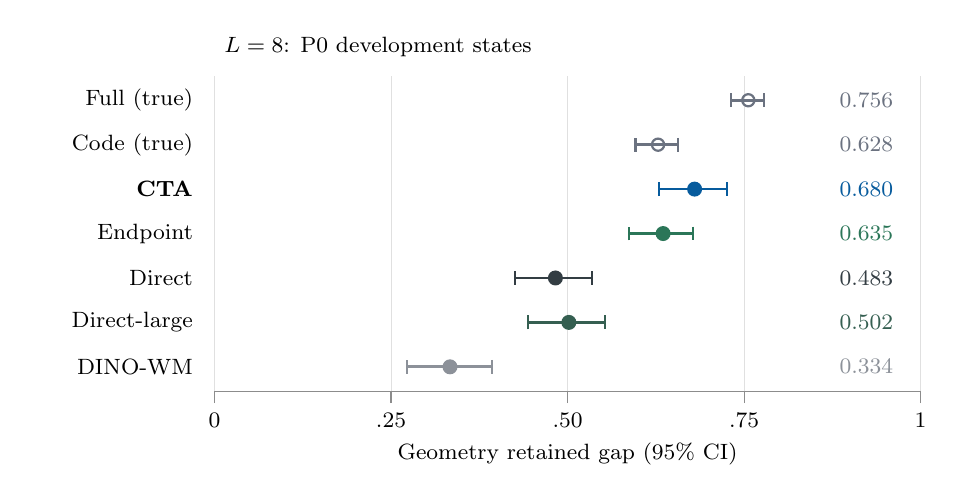
\begin{tikzpicture}
\definecolor{ctaplotblue}{HTML}{075B9D}
\definecolor{ctaplotgreen}{HTML}{2B7658}
\definecolor{ctaplotdeepgreen}{HTML}{355F51}
\definecolor{ctaplotdark}{HTML}{333D43}
\definecolor{ctaplotpriv}{HTML}{6B7280}
\definecolor{ctaplotdino}{HTML}{8C9199}
\begin{axis}[
  width=0.87\linewidth,
  height=2.20in,
  xmin=0, xmax=1,
  ymin=0.45, ymax=7.55,
  xtick={0,0.25,0.5,0.75,1},
  xticklabels={0,.25,.50,.75,1},
  ytick={7,6,5,4,3,2,1},
  yticklabels={Full (true),Code (true),\textbf{CTA},Endpoint,Direct,Direct-large,DINO-WM},
  font=\fontsize{8}{9}\selectfont,
  tick label style={font=\fontsize{8}{9}\selectfont},
  yticklabel style={text width=0.78in,align=right},
  xlabel={Geometry retained gap (95\% CI)},
  xlabel style={font=\fontsize{8}{9}\selectfont,yshift=1pt},
  axis x line*=bottom,
  axis y line*=left,
  y axis line style={draw=none},
  axis line style={black!45,line width=0.4pt},
  tick align=outside,
  tick style={black!45,line width=0.4pt},
  ytick style={draw=none},
  xmajorgrids=true,
  grid style={black!12,line width=0.3pt},
  clip=false,
  enlarge y limits=false,
]
\node[anchor=south west,font=\fontsize{8}{9}\selectfont]
  at (rel axis cs:0,1.03) {$L=8$: P0 development states};
\addplot[
  only marks,mark=o,mark options={fill=white,line width=0.8pt},mark size=2.2pt,color=ctaplotpriv,line width=1.0pt,
  error bars/.cd,x dir=both,x explicit,
  error bar style={line width=1.0pt},
  error mark options={rotate=90,mark size=2.5pt,line width=0.8pt}
] coordinates {(0.756003,7) +=(0.022116,0) -=(0.024909,0)};
\node[anchor=east,text=ctaplotpriv,font=\fontsize{8}{9}\selectfont]
  at (axis cs:0.975,7) {0.756};
\addplot[
  only marks,mark=o,mark options={fill=white,line width=0.8pt},mark size=2.2pt,color=ctaplotpriv,line width=1.0pt,
  error bars/.cd,x dir=both,x explicit,
  error bar style={line width=1.0pt},
  error mark options={rotate=90,mark size=2.5pt,line width=0.8pt}
] coordinates {(0.628188,6) +=(0.028753,0) -=(0.031862,0)};
\node[anchor=east,text=ctaplotpriv,font=\fontsize{8}{9}\selectfont]
  at (axis cs:0.975,6) {0.628};
\addplot[
  only marks,mark=*,mark size=2.2pt,color=ctaplotblue,line width=1.0pt,
  error bars/.cd,x dir=both,x explicit,
  error bar style={line width=1.0pt},
  error mark options={rotate=90,mark size=2.5pt,line width=0.8pt}
] coordinates {(0.679928,5) +=(0.045792,0) -=(0.050448,0)};
\node[anchor=east,text=ctaplotblue,font=\fontsize{8}{9}\selectfont]
  at (axis cs:0.975,5) {0.680};
\addplot[
  only marks,mark=*,mark size=2.2pt,color=ctaplotgreen,line width=1.0pt,
  error bars/.cd,x dir=both,x explicit,
  error bar style={line width=1.0pt},
  error mark options={rotate=90,mark size=2.5pt,line width=0.8pt}
] coordinates {(0.635334,4) +=(0.042480,0) -=(0.047753,0)};
\node[anchor=east,text=ctaplotgreen,font=\fontsize{8}{9}\selectfont]
  at (axis cs:0.975,4) {0.635};
\addplot[
  only marks,mark=*,mark size=2.2pt,color=ctaplotdark,line width=1.0pt,
  error bars/.cd,x dir=both,x explicit,
  error bar style={line width=1.0pt},
  error mark options={rotate=90,mark size=2.5pt,line width=0.8pt}
] coordinates {(0.482833,3) +=(0.052255,0) -=(0.057436,0)};
\node[anchor=east,text=ctaplotdark,font=\fontsize{8}{9}\selectfont]
  at (axis cs:0.975,3) {0.483};
\addplot[
  only marks,mark=*,mark size=2.2pt,color=ctaplotdeepgreen,line width=1.0pt,
  error bars/.cd,x dir=both,x explicit,
  error bar style={line width=1.0pt},
  error mark options={rotate=90,mark size=2.5pt,line width=0.8pt}
] coordinates {(0.501882,2) +=(0.051130,0) -=(0.057361,0)};
\node[anchor=east,text=ctaplotdeepgreen,font=\fontsize{8}{9}\selectfont]
  at (axis cs:0.975,2) {0.502};
\addplot[
  only marks,mark=*,mark size=2.2pt,color=ctaplotdino,line width=1.0pt,
  error bars/.cd,x dir=both,x explicit,
  error bar style={line width=1.0pt},
  error mark options={rotate=90,mark size=2.5pt,line width=0.8pt}
] coordinates {(0.333532,1) +=(0.059297,0) -=(0.061128,0)};
\node[anchor=east,text=ctaplotdino,font=\fontsize{8}{9}\selectfont]
  at (axis cs:0.975,1) {0.334};
\end{axis}
\end{tikzpicture}

\caption{\textbf{Ranking on the same P0 decision banks.} $L=8$, $K=8$, 200 development roots. Horizontal bars are 95\% root-bootstrap intervals. Hollow grey points use actual future information; filled points are deployable scorers. DINO-WM is an external checkpoint reference with unmatched observation/training details.}
\label{fig:ranking}
\end{figure}
\begin{table}[t]
\centering\small
\begin{tabular}{lrr}
\toprule
Paired RG difference & Estimate & 95\% CI \\
\midrule
CTA $-$ END & +.045 & [.011,.079] \\
CTA $-$ DIR & +.197 & [.153,.241] \\
CTA $-$ DIR-large & +.178 & [.138,.220] \\
CTA $-$ DINO-WM & +.346 & [.294,.398] \\
\bottomrule
\end{tabular}
\caption{Paired root-bootstrap contrasts for \cref{fig:ranking}. The last comparison retains the external-baseline caveats.}
\label{tab:pairedrank}
\end{table}

FULL reaches .756 [.731,.778], while CODE reaches .628 [.596,.657]. Predicted CTA exceeds CODE's point estimate. Thus the diagnostic tiers are not a monotone oracle-to-code-to-prediction degradation ladder. In particular, the continuous predictive mean is a different reader input from a realized quantized source code; smoothing is a possible explanation, not a demonstrated mechanism. These diagnostics locate a discrepancy for further study rather than proving that prediction recovers information lost by compression.

\subsection{RQ2: closed-loop behavior and computation}
\label{sec:closed}
\Cref{tab:closed} reports historical runs using the old batched proposal sampler. Within each run, arms share the policy, candidate count, horizon, and seed mapping. Their visited states diverge after different selections. CTA succeeds in 140/200 episodes at $L=8$, versus 138 for END, 135 for DIR, and 136 for DINO-WM. The paired learned-arm differences have broad intervals crossing zero (\cref{tab:closeddiff}). CTA's +9-point difference over P0 is more promising, but cannot establish superiority over the learned alternatives.

\begin{table}[t]
\centering\small
\setlength{\tabcolsep}{4pt}
\begin{tabular}{lrrrr}
\toprule
& \multicolumn{2}{c}{$L=8$} & \multicolumn{2}{c}{$L=15$} \\
Arm & Success & Score & Success & Score \\
\midrule
P0 & 122/200 & .961 & 103/200 & .911 \\
GEOM (privileged) & 160/200 & .970 & 149/200 & .948 \\
CTA & 140/200 & .960 & 121/200 & .930 \\
END & 138/200 & .956 & 108/200 & .936 \\
DIR & 135/200 & .973 & 103/200 & .920 \\
DINO-WM & 136/200 & .974 & 112/200 & .932 \\
\bottomrule
\end{tabular}
\caption{\textbf{Historical development control, old proposal protocol.} One training seed; same 200 development roots at each horizon. Score uses maximum post-action coverage (excluding reset coverage), divided by .95 and clipped at one. Numerical sensitivity in \cref{sec:repro} limits reproducibility. Horizon training mixtures differ, so this is not a pure horizon ablation.}
\label{tab:closed}
\end{table}
\begin{table}[t]
\centering\small
\setlength{\tabcolsep}{3pt}
\begin{tabular}{lcc}
\toprule
Paired success difference & $L=8$ & $L=15$ \\
\midrule
CTA $-$ P0 & +9 [1,17.5] & +9 [1,17] \\
CTA $-$ END & +1 [$-$7.5,9.5] & +6.5 [$-$2.5,15.5] \\
CTA $-$ DIR & +2.5 [$-$5.5,10.5] & +9 [.5,17.5] \\
CTA $-$ DINO-WM & +2 [$-$6,10] & +4.5 [$-$4.5,13.5] \\
\bottomrule
\end{tabular}
\caption{Percentage-point differences and paired 95\% root-bootstrap intervals for \cref{tab:closed}. Exact McNemar $p$ for CTA--DIR at $L=15$ is .05045 despite the bootstrap interval excluding zero; no unqualified significance claim is made. Complete $p$ values are in the supplement.}
\label{tab:closeddiff}
\end{table}

At $L=15$, CTA reaches 121 successes compared with DIR's 103. However, the change in their success difference between horizons is +6.5 points with interval [$-$4,17], and training data also change. This does not establish horizon robustness. Mean-score contrast intervals cross zero, and CTA does not lead the $L=8$ mean-score column. A binary success gain and improved average coverage are distinct claims.

\paragraph{Component timing.}
\Cref{tab:timing} reports archived synchronized measurements on an H100 3g.40gb MIG instance: ten initial states, three warmups and ten repeats per state for scorer/context timing (one warmup and three repeats for policy sampling). CTA's predictor/reader takes 4.11ms for one goal view and 16.87ms for sixteen. The latter are views of one target, not distinct semantic tasks. For our arms, the table excludes shared encoding; DINO-WM includes its own encoding, rollout, and cost. Precision is not fully matched. Therefore 4.11 versus 28.96ms is not a whole-planner speedup. The common policy sampler takes approximately 765ms and dominates this workload. End-to-end latency, memory, and matched-precision Pareto comparisons remain unmeasured.

\begin{table}[t]
\centering\small
\begin{tabular}{lrr}
\toprule
Component ($K=8$), median ms & $G=1$ & $G=16$ \\
\midrule
Shared DINOv2/PCA context & 6.49 & 6.48 \\
CTA predictor + reader & 4.11 & 16.87 \\
END predictor + reader & 4.52 & 23.40 \\
DIR scorer & 2.54 & 26.81 \\
DINO-WM own encode + rollout + cost & 28.96 & 29.07 \\
Common policy sampling & 765.33 & 765.33 \\
\bottomrule
\end{tabular}
\caption{Component measurements with deliberately explicit scope. Our scorer rows exclude the shared context encoder and all rows exclude simulator execution. Rows with different scopes must not be interpreted as total-planner comparisons.}
\label{tab:timing}
\end{table}

\subsection{RQ3: source, prediction, and objective failures}
\label{sec:diagnostics}
\paragraph{Longer-horizon prediction gap.}
On 1,476 selection banks from 100 separate development roots at $L=15$, CODE achieves .667 [.608,.719] but predicted CTA reaches .374 [.265,.478] (\cref{fig:bottleneck}). The .294 point difference \mbox{identifies} prediction/readout as a concrete bottleneck for this configuration. It is not a paired-confidence result, and selection data cannot provide an independent generalization test. The $L=8$ selection population has a different mixture and should not be used as a matched horizon comparison.

\begin{figure}[t]
\centering% Transcribed saved root-bootstrap estimates; provenance in evidence_data.json.
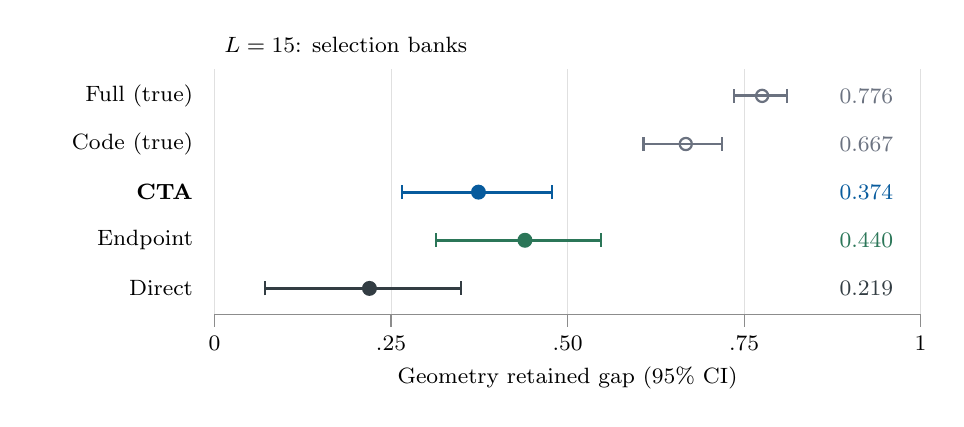
\begin{tikzpicture}
\definecolor{ctaplotblue}{HTML}{075B9D}
\definecolor{ctaplotgreen}{HTML}{2B7658}
\definecolor{ctaplotdeepgreen}{HTML}{355F51}
\definecolor{ctaplotdark}{HTML}{333D43}
\definecolor{ctaplotpriv}{HTML}{6B7280}
\definecolor{ctaplotdino}{HTML}{8C9199}
\begin{axis}[
  width=0.87\linewidth,
  height=1.85in,
  xmin=0, xmax=1,
  ymin=0.45, ymax=5.55,
  xtick={0,0.25,0.5,0.75,1},
  xticklabels={0,.25,.50,.75,1},
  ytick={5,4,3,2,1},
  yticklabels={Full (true),Code (true),\textbf{CTA},Endpoint,Direct},
  font=\fontsize{8}{9}\selectfont,
  tick label style={font=\fontsize{8}{9}\selectfont},
  yticklabel style={text width=0.78in,align=right},
  xlabel={Geometry retained gap (95\% CI)},
  xlabel style={font=\fontsize{8}{9}\selectfont,yshift=1pt},
  axis x line*=bottom,
  axis y line*=left,
  y axis line style={draw=none},
  axis line style={black!45,line width=0.4pt},
  tick align=outside,
  tick style={black!45,line width=0.4pt},
  ytick style={draw=none},
  xmajorgrids=true,
  grid style={black!12,line width=0.3pt},
  clip=false,
  enlarge y limits=false,
]
\node[anchor=south west,font=\fontsize{8}{9}\selectfont]
  at (rel axis cs:0,1.03) {$L=15$: selection banks};
\addplot[
  only marks,mark=o,mark options={fill=white,line width=0.8pt},mark size=2.2pt,color=ctaplotpriv,line width=1.0pt,
  error bars/.cd,x dir=both,x explicit,
  error bar style={line width=1.0pt},
  error mark options={rotate=90,mark size=2.5pt,line width=0.8pt}
] coordinates {(0.775561,5) +=(0.035462,0) -=(0.040078,0)};
\node[anchor=east,text=ctaplotpriv,font=\fontsize{8}{9}\selectfont]
  at (axis cs:0.975,5) {0.776};
\addplot[
  only marks,mark=o,mark options={fill=white,line width=0.8pt},mark size=2.2pt,color=ctaplotpriv,line width=1.0pt,
  error bars/.cd,x dir=both,x explicit,
  error bar style={line width=1.0pt},
  error mark options={rotate=90,mark size=2.5pt,line width=0.8pt}
] coordinates {(0.667457,4) +=(0.051826,0) -=(0.059787,0)};
\node[anchor=east,text=ctaplotpriv,font=\fontsize{8}{9}\selectfont]
  at (axis cs:0.975,4) {0.667};
\addplot[
  only marks,mark=*,mark size=2.2pt,color=ctaplotblue,line width=1.0pt,
  error bars/.cd,x dir=both,x explicit,
  error bar style={line width=1.0pt},
  error mark options={rotate=90,mark size=2.5pt,line width=0.8pt}
] coordinates {(0.373872,3) +=(0.103686,0) -=(0.108626,0)};
\node[anchor=east,text=ctaplotblue,font=\fontsize{8}{9}\selectfont]
  at (axis cs:0.975,3) {0.374};
\addplot[
  only marks,mark=*,mark size=2.2pt,color=ctaplotgreen,line width=1.0pt,
  error bars/.cd,x dir=both,x explicit,
  error bar style={line width=1.0pt},
  error mark options={rotate=90,mark size=2.5pt,line width=0.8pt}
] coordinates {(0.439646,2) +=(0.107962,0) -=(0.126243,0)};
\node[anchor=east,text=ctaplotgreen,font=\fontsize{8}{9}\selectfont]
  at (axis cs:0.975,2) {0.440};
\addplot[
  only marks,mark=*,mark size=2.2pt,color=ctaplotdark,line width=1.0pt,
  error bars/.cd,x dir=both,x explicit,
  error bar style={line width=1.0pt},
  error mark options={rotate=90,mark size=2.5pt,line width=0.8pt}
] coordinates {(0.219485,1) +=(0.129109,0) -=(0.148156,0)};
\node[anchor=east,text=ctaplotdark,font=\fontsize{8}{9}\selectfont]
  at (axis cs:0.975,1) {0.219};
\end{axis}
\end{tikzpicture}

\caption{\textbf{A prediction bottleneck on $L=15$ selection data.} $K=8$, 1,476 banks, 100 roots (2000--2099). Source CODE retains substantially more geometry improvement than predicted CTA. This is a development diagnostic, separate from the P0 evaluation population in \cref{fig:ranking}.}
\label{fig:bottleneck}
\end{figure}

\paragraph{Rare native-success crossings.}
Crossing banks, where candidate zero fails within the chunk but at least one sibling succeeds, are rare on logged P0 states: 58/5,558 at $L=8$ and 35/3,249 at $L=15$. CTA selects a successful candidate in .793 and .371 of these banks, respectively; source CODE captures .897 and .914. The geometry oracle captures .983 and 1.000, so its endpoint proxy is informative on these crossings. The weaker predicted capture points to forecast/readout fidelity; different objective definitions alone do not establish widespread utility mismatch. Small denominators and downstream recovery limit translation to episode success. Ranking can improve many decisions without improving the few that determine termination. A native-hit continuation with matched CTA/END/DIR controls has been prepared, but no trained checkpoint or result is included here.

\paragraph{Predictability can destroy distinctions.}
An earlier, separate co-design pilot penalized source codes that were difficult for a predictor copy, frozen within each source-update block, to predict; source and predictor updates alternated. Increasing its weight from zero to .1 reduced prediction cross-entropy from .558 to .086 nats/token, but source RG fell from .706 to .458 (paired difference $-.248$ [$-.297,-.200$]). Token perplexity fell from 131.2 to 1.37 and sibling distinctness from .765 to .206. This is evidence of collapse in the tested pilot, not a universal rejection of co-design. It demonstrates why low forecast loss alone is insufficient evidence of a useful decision target. The pilot uses an earlier model and data regime, not the final v2 control comparison.

\subsection{Numerical reproducibility and validity}
\label{sec:repro}
The old proposal protocol changes sampled chunks with batch grouping. With the same 200 $L=15$ roots and weights, two evaluations report P0 successes 100 and 103, but 43 roots change success status; GEOM has 29 such flips. Net counts therefore hide large episode-level disagreement. On one inspected root, grouping the policy batch from one to four changes initial actions by up to .0563 world units. This demonstrates one source of sensitivity, without fully attributing every discrepancy.

Canonical policy sampling fixes denoising microbatch shapes and candidate-prefix construction. A bounded P0 check for root 2205 alone versus grouped with root 2206 passes: $K=1,8,16$ action prefixes match exactly, discrete decision fields agree, and coverage differs by at most $3.33\times10^{-16}$ under an absolute tolerance of $10^{-12}$. Scorer-shape handling is prepared in the continuation source but remains unqualified; the check has not certified every learned arm, root, or backend. Canonical samples also differ from historical ones. Consequently, \cref{tab:closed} remains an explicitly historical result; it is not relabeled as a validated canonical evaluation. The next control result must be collected under the qualified protocol rather than inferred from archived counts.
